\section{Basics}

	\subsection{RS-485 [AK]}
		RS-485 was created by the Telecommunications Industry Association and Electronic Industries Alliance (TIA/EIA) to overcome the disadvantages of the RS-232 serial communication device. It is used in two-wire data transfer.  Via RS-485 serial communication protocol, the master can communicate up to 32 devices via a wire bus connection as shown in the diagram
	
		\footnotetext{ Figure 1 source: https://www.advantech.com/en/resources/white-papers/02cb2f4e-4fb2-4a87-be3b-508325bd61d6}
		\begin{figure}[H]
			\centering
			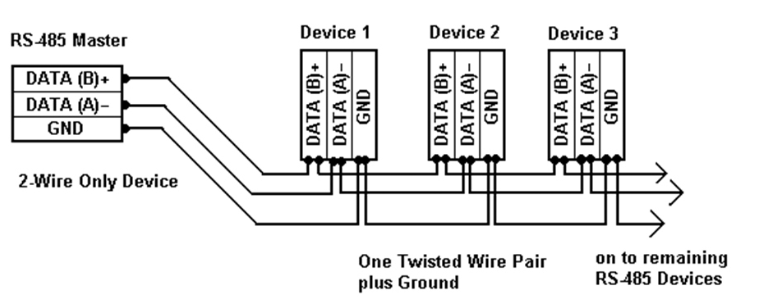
\includegraphics{assets/AK-rs485-masterslave.png}
			\caption{RS-485 Master Slave Connection}
			\label{fig:modbus-master-slave}
		\end{figure}
	
	
		The frame structure of RS-485 is mentioned in the below image. Data transfer will start from High to low pulse (Mark) and then followed by 8 bits of data and then as per the configuration it will use odd parity or even parity. At last low to high pulse (Space) for ending the data transmission.
	
		\begin{figure}[H]
			\centering
			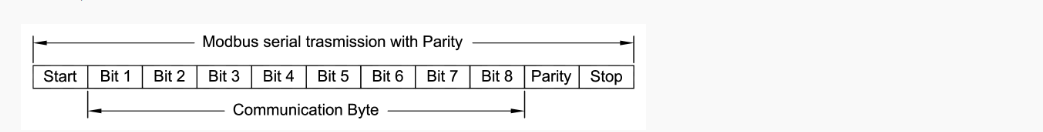
\includegraphics{assets/AK-data-frame-transmission.png}
			\caption{Data Frame Structure Transmission}
		\end{figure}
	
		\footnotetext{ Figure 2 source: https://web-plc.com/blog/2017/06/01/rtu-modbus}
		
		\subsection{Modbus data-link layer [BP]}
		\label{sec:modbus-data-link-layer}
		The following section of this report describes how the Modbus data-link layer works. Modbus works on the data-link layer to trade frames between two device, in the previous part we focused on the electrical part here we will focus on the concept on frames exchange and on frames. 
			
			\subsubsection{The protocol}
				
				\begin{figure}[H]
					\centering
					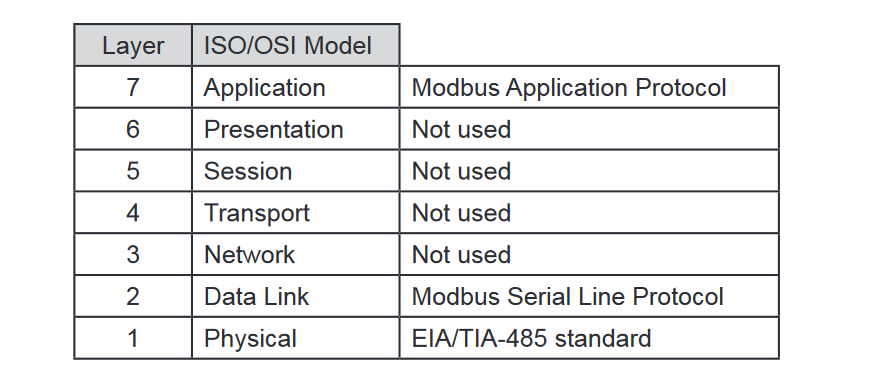
\includegraphics[width=0.7\linewidth]{assets/data-link-layer.png}\qquad
					\caption{Layer where Modbus works~\cite{Modbus-protocol}}
						
					\label{fig:modbus-data-link}
				\end{figure}
			
				The Modbus protocol works on the layer 1, 2 and 7, so there is no interaction between the frame which is sent by the device and how the frame is recieved on the application, that's why it's important to know how this protocol works.
			
				\begin{figure}[H]
					\centering
					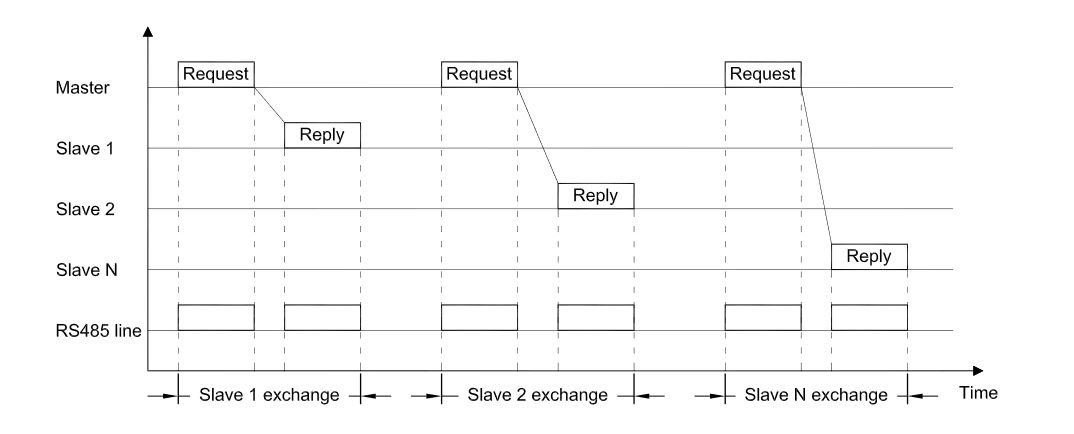
\includegraphics[width=0.9\linewidth]{assets/master-slave-communication.png}\qquad
					\caption{Master slave communication~\cite{Modbus-protocol}} 
					\label{fig:modbus-master-slave-comm}
				\end{figure}
				
				Modbus is based on a master slave communication, the device is consider as the master and send requests to the sensor which is consider as a slave and answer to the request. Each sensor can send informations to multiple device and device can ask different sensors. 
				
			\subsubsection{The frame}
			
				\begin{figure}[H]
					\subfloat[The frame in bytes]{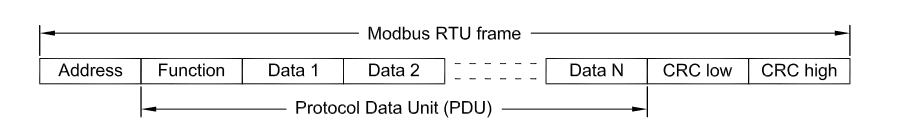
\includegraphics[width=0.5\linewidth]{assets/frame-in-bytes.png}}\qquad
					\subfloat[The frame time]{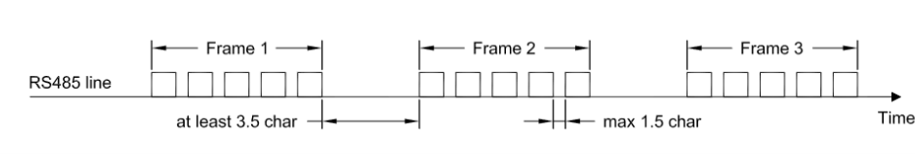
\includegraphics[width=0.5\linewidth]{assets/frame-time.png}}
					\caption{Typical frame~\cite{Modbus-protocol}}
					\label{fig:hw-components}
				\end{figure}
				
				Each frame consists of one byte of addressing to connect to the sensor, one byte of protocol type, as many bytes as necessary for data transfer and two bytes of error control that are important to ensure the integration of communication. Frames are sent in regular time intervals to ensure the integrity of the link (if a delay appears is that a frame is missing).
				
				Traditionally, sensor addresses are~\cite{Modbus-protocol}:
				\begin{itemize}
					\item 0 broadcast for slave
					\item 1 – 247 unicast
					\item 248 – 255 impossible (reserved for the manufacturer)
				
				\end{itemize}
				
				In details, there are two types of bytes, one with a parity cock and one without, this does not change much because it is just replaced by a stop bit.
				
				\begin{figure}[H]
					\subfloat[A byte with parity]{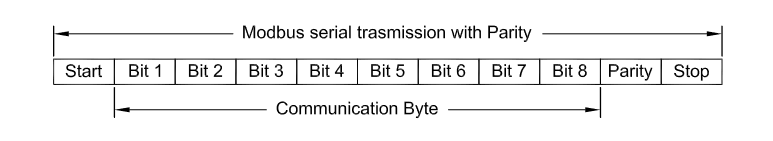
\includegraphics[width=0.5\linewidth]{assets/byte-parity.png}}\qquad
					\subfloat[A byte without parity]{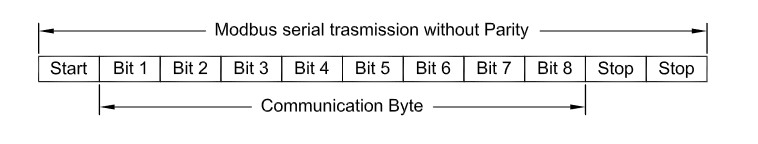
\includegraphics[width=0.5\linewidth]{assets/byte-without-parity.png}}
					\caption{The byte in details~\cite{Modbus-protocol}}
					\label{fig:byte-parity5}
				\end{figure}
		
	\subsection{ESP32 [DS]}
		\label{sec:esp32}
		
		The ESP32 microcontroller family, developed by Espressif System, is very famous for providing best features which are perfectly suited wild range of IoT projects and application. There are many different microcontroller are offered by Espressif, However for this project, ESP32 family’s Microcontroller are well suited as its key features are a dual-core Xtensa LX6 processor, integrated Wi-Fi and Bluetooth capabilities, a robust set of peripherals, and scalable memory options. Here, we've chosen the ESP 32-WROOM 32E microcontroller, embedded in the ESP32 Olimex board,  from the ESP32 family.
		
		\subsubsection{ESP32 WROOM 32 E}
			Since we wish to access our data via a MQTT broker, a variety of connectivity options are important considerations when selecting a device. Here, we've chosen the ESP 32-WROOM 32E micro controller(Depicted on the left side) on the  from the ESP32 family. This has an Ethernet connector, WiFi, and Bluetooth chip built right in.We decided on this ESP32-WROOM 32E rather than an Arduino since an Arduino requires the inclusion of wifi and bluetooth modules. It also has more integrated components, such as an antenna and flash memory, and is quite affordable. These points all satisfy our requirements and are most appropriate for our project.
		
			\begin{figure}[H]
				\centering
				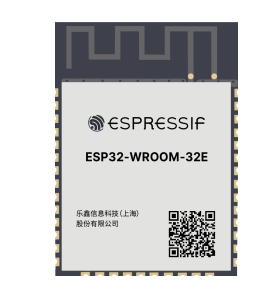
\includegraphics[width=0.4\linewidth]{assets/DS-esp32.png} 
				\caption{ESP32 WROOM 32E processor~\cite{esp-32-package}.}
			\end{figure}
		
		\subsubsection{Dual Core- Processor}
			The module is chipped with dual-core Xtensa LX6 processor, this configuration gives ESP32 to work on different task at a same time with correct output on two processing units. Dual core feature provide upgraded overall performance and multitasking capability. It has clock frequency range from 80 MHz to 240 MHz. This clock frequency is editable by the operator. 
		
		\subsubsection{Pin Configuration}
			\begin{figure}[H]
				\centering
				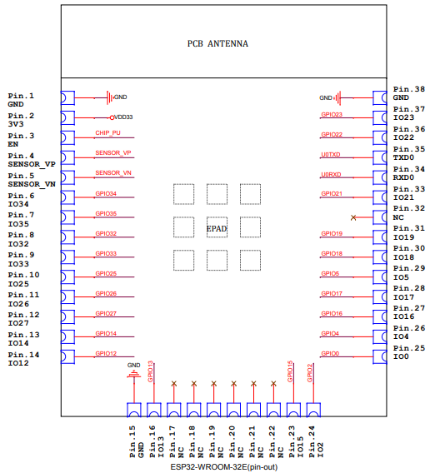
\includegraphics[width=0.4\linewidth]{assets/DS-esp32-pin.png} 
				\caption{Pin configuration~\cite{esp-32-package}.}
			\end{figure}
			This module has a diverse pin configuration. Its has 40 GPIO(General Purpose Input Output) pins(e.g., GPIO04, GPIO12), which gives versatile Analog and Digital communication feature. Furthermore, it also has UART pins (TX0,RX0), by which the serial communication (e.g., RS485 modbus) become very easy. It also have ADC pins, PWM pins, boot and Reset pins, I2C pins and SPI pins.
		
		
		\subsubsection{Wireless Connectivity}
			This processor has inbuilt Wi-Fi(802.11b/g/n), which can operate as station mode and access point mode. Also, it support WiFi communication security with WPA/WPA2. During transmission of data, it can do encryption in order to ensure data security. With WiFi it also have inbuilt Bluetooth support. 
		
		\subsubsection{Memory Configuration}
			The ESP32 WROOM 32E is devided into two different memory type, SRAM \& Flash memory. SRAM(Static Random-Access Memory) it used for storing temporary data, high speed and inorder to improve overall performance of module. On the other hand, Flash Memory is Non-volatile type of memory, where the real program code, firmware and data are stored.
		
	\subsection{ESPHome Introduction [AK]}
		Several options were available for flashing the ESP-32 device like Arduino-IDE, ESP-Home, Platform-IO, etc. To decide which platform, you require you need to consider your application like what purpose you want to solve. Our application was to connect with Text sensors like MQTT subscribers, Modbus, and many more, and ESPHome can do that. Also, ESPHome has an advantage in that it is a web-based interface so you can connect to any device without actually installing that application.
	
		\begin{figure}[H]
			\centering
			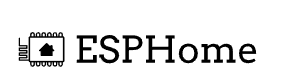
\includegraphics{assets/AK-esphome.png}
			\caption{ESPHome Firmware Logo}
			\label{fig:example}
		\end{figure}
	
		\footnotetext{ Figure 1 source: https://esphome.io}
	
		\setlength{\parindent}{0pt}
	
		ESPHome uses YAML (Yet Another Markup Language) for configuration, making it accessible to users without extensive programming experience. We can start with the ESPHome in several ways, like Using a Command line, From the Home assistant, and using a Docker container. Due to ESPHome’s inherent Modbus compatibility, you can link to any Modbus network and interact with any Modbus-compatible sensor. One of ESPHome's major benefits over other firmware devices is that it is an open-source platform with a vibrant and expanding community of users. If you run into any issues, you can always reach out to the community for help. Furthermore, over-the-air upgrades are supported by ESPHome, enabling users to access the device virtually.
		
	\subsection{MQTT [MS]}
		Message Queuing Telemetry Transport (MQTT) is open-source, lightweight, and publish-subscribe
		messaging protocol. Primarily designed for the communication among the devices those contain the
		resource.
		
		\subsubsection*{Features}
			\begin{description}
				\item[Publish-Subscribe-Architecture]  It uses publish-subscribe model, which allows the devices to act as
				publishers or subscribers.
				\item[Broker-Based Communication]  MQTT communication relies on a broker that acts as a mediator
				between publishers and subscribers. The broker efficiently manages message routing to ensure
				messages reach the intended recipients.
				\item[Topics]  Communication in MQTT uses topics, hierarchical strings used to categorize messages.
				Subscribers express interest in specific topics, and publishers send messages to these topics.
				\item[\acf{QoS} Levels] MQTT provides configurable levels of reliability (QoS Levels 0, 1,
				2)
				\item[Security Features] Transport Layer Security (TLS) encryption, can be implemented to secure MQTT
				communication.
				\item[Retained messages] the broker stores a last known good value for new subscribers
				\item[Persistent sessions] the broker stores messages on behalf of a subscriber that is temporarily offline
				\item[Heartbeats]  if the broker does not receive a PINGREQ for some time, it will close the connection and
				send the Last Will and Testament (LWT)
				\item[\acf{LWT}] A predefined message sent to all subscribers by the broker in case a
				device stops responding.
			\end{description}
	
	\subsection{DEIF MIC-2 MKII [MS]}
		DEIF MIC-2 MKII is a multi-instrument used to monitor and control the operations. The unit
		continuously updates metering results and allows users online access to monitor. It has the
		capability of logging from single low voltage to multiple high voltage parameters. All
		metering data and setting parameters can be accessed by using the front panel keys or with the
		communication port. Setting parameters are stored in the EEPROM.
		
		\begin{figure}[H]
			\centering
			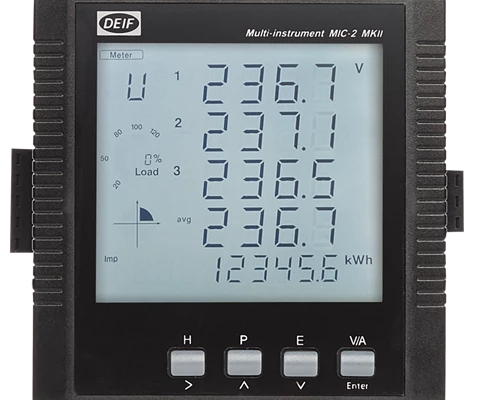
\includegraphics[width=0.6\linewidth]{assets/MS-deif.png}
			\caption{DEIF MIC 2 MKII~\cite{deif-mk2}}
			\label{fig:deif-mic-mk2}
		\end{figure}
		
		\subsubsection*{Features}
			\begin{itemize}
				\item Multiple connected devices- Uses RS-485 Modbus communication (Up to 32 devices
				can be connected on a RS485 bus)
				\item Customized alarm settings- facilitate to customize upto16 different parameters
				\item Password protected setting- Counter reset and change of settings can be password-
				protected
				\item Display- Large LCD screen with white backlight
				\item Control and Monitoring- It provides a user interface for operators to monitor the
				parameters and control its operation.
				\item Communication- the instrument support various communication modules - Ethernet
				(Modbus TCP, HTTP, SMTP), Profibus DP
				\item Remote Access- Remote monitoring and control capabilities allow users to access and
				manage the generator set from a distance.
				\item Inputs and Outputs- Optional Input and Output modules - Relay , Analogue I/O,
				Digital I/O
				\item Data Logging-It may include data logging features, allowing operators to analyze
				historical performance data and identify trends.
				\item Customizable Configurations- Users may have the ability to configure the controller to
				meet specific application requirements, adapting it to different measurements and
				operational scenarios.
			\end{itemize}
	
	
